\documentclass[12pt,a4paper]{article}
\usepackage[utf8]{inputenc}
\usepackage[T1]{fontenc}
\usepackage[dutch]{babel}
\usepackage{amsmath}
\usepackage{amsfonts}
\usepackage{amssymb}
\usepackage{graphicx}
\usepackage{algpseudocode}
\usepackage{algorithm}
\usepackage{fullpage}
\usepackage{subfigure}


\author{Estelle Severs, Maarten Magits}
\title{Studentencursus TMI}
\begin{document}
	%TODO Screenshots van pseudocode vervangen door effectieve pseudocode. 
	\maketitle
	\tableofcontents
	\section{Introductie}
	Toepassingen van de informatica (TMI) wordt ook wel Computationele geometrie (CG) genoemd.
	In het algemeen handelt dit domein over het berekenen en manipuleren van geometrische entiteiten/vormen en een oplossing te vinden voor geometrische problemen.
	Er vallen twee subdomeinen te onderscheiden:
	\begin{enumerate}
		\item \textbf{Combinatorial CG}: De studie van concrete objecten. Behandelt de discrete ruimte.
		\item \textbf{Numerical CG}: De studie van curves en functies. Eerder abstract.
	\end{enumerate}
	Dit OPO gaat grotendeels over de Combinatorial CG met slects een klein deeltje Numerical CG. In de slides volgen hier nog wat voorbeelden op, maar je kan ook gewoon de hoofdstukken beginnen bekijken voor goeie voorbeelden. 
	
	In deze cursus zullen we de volgende stappen telkens volgen voor het opmaken van een algoritme: 
	\begin{enumerate}
		\item Aanvankelijk negeren we de speciale gevallen. Op deze manier maken we een eerste versie van het algoritme
		\item Nu passen we ons algoritme aan op de speciale gevallen. Dit kan met (domme) if-then-else testen zullen we eerder vermijden. We willen het algoritme zo aanpassen zodat de speciale gevallen gewoon opgelost geraken. 
		\item Dan zal je het effectieve algoritme implementeren!
	\end{enumerate}
	
	
	\section{Les 1: Convex Omhullende}
	Het deeltje over convex omhullende begint met wat basis definities over wat dit eigenlijk is. Er is daarna ook een figuur om het volledig duidelijk te maken. 
		\begin{description}
			\item[Convexe verzameling] Een vorm (shape) of verzameling (set) is convex indien voor elk paar punten die tot de verzameling behoren, het lijnsegment dat beide punten verbindt ook behoort tot die verzameling. 
			\item[Convex omhullende] Voor een deelverzameling van het vlak, is de convex omhullende de kleinst mogelijke convexe vorm die de hele deelverzameling bevat. 
		\end{description}
	Om je een idee te geven van het belang van zo een convex omhullende, geven we ook wat applicaties. Daarna zullen we ingaan op de algoritmes om ze te bepalen. 
		\begin{itemize}
			\item Als een verzameling punten staat voor een aantal obstakels, zal een robotarm het pad 	errond kiezen volgens de convex omhullende. 
			\item We kunnen bij het detecteren of twee figuren overlappen, de convex omhullende berekenen en dan zien of deze vormen al overlappen. Als dat niet het geval is, zullen de vormen zelf ook niet overlappen. 
			\item Om het puntenpaar te vinden dat het verst van elkaar gelegen is in een verzameling, is het relevant de convex omhullende te bepalen aanegzien alle punten die het verste van elkaar zitten in de verzameling ook op de convex omhullende zullen liggen. 
		\end{itemize}
	We gaan nu het bepalen van de convex omhullende bespreken. We gaan hier gebruik maken van een input aan punten \(P = {p_1, p_2, p_3, ..., p_n}\). De output zal de punten op de convexe veelhoek zijn geordend in klokwijzerzin. We zullen de convex omhullende noteren als $CH(P)$.
	
	
	\subsection{Brute Force algoritme}
	Het brute-force algoritme gaat voor elk paar aan punten nakijken of alle andere punten aan de rechterkant liggen. Als dit het geval is, is dit deel van de convexe veelhoek en wordt deze toegevoegd aan de lijst van edges E. De laatste stap zal er nog eens over de edges gegaan worden om deze in de juiste volgorde te steken. 
	De input is in dit geval een set punten P in een vlak. De output is dan een list $\mathcal{L}$ met de vertices van $CH(P)$ in wijzerzin. Hieronder is de pseudocode voor het algoritme
	\begin{figure}[h]
		\centering
		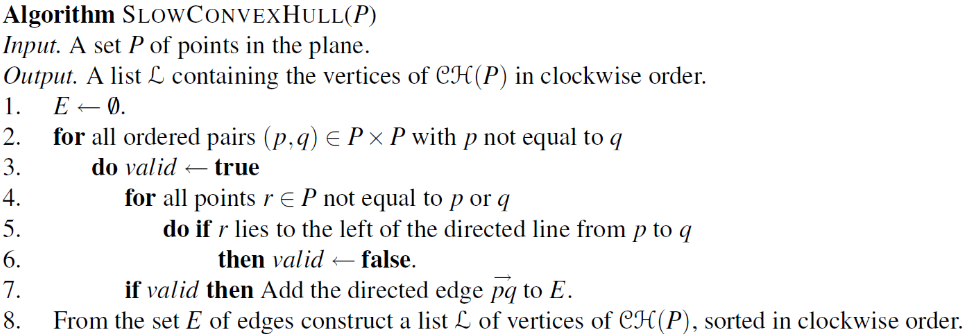
\includegraphics[width=0.9\linewidth]{afbeeldingen/slowconvexhull}
		\label{fig:slowconvexhull}
	\end{figure}
	
	De eerste lus zal $n^2$ keer lopen, gezien het voor elk paar hetgeen in de lus zal uitvoeren. In de lus zelf zal er nog eens over de punten gelopen worden om te kijken of deze allemaal rechts liggen van het gegeven punt, wat nog een $n$ keer zal lopen. De tijdscomplexiteit van dit algoritme is dus $O(n^3)$. 
	
	Naast het feit dat het algoritme helemaal niet efficiënt is, zijn er ook wat problemen in verband met de nauwkeurigheid van het berekenen of zo een punt links of rechts licht van een ander punt. Het kan zijn dat hierdoor punten fout worden bepaald terwijl ze wel links liggen van een edge. Een ander probleem is wanneer er meerdere punten op een lijn liggen, dit is dan een speciaal geval maar hier zou extra rekening mee gehouden moeten worden, het algoritme zal hier niet automatisch mee omgaan. Dit algoritme is dus duidelijk niet al te efficiënt en er zijn een paar gevallen waarbij het zelfs foute beslissingen kan maken. 
	
	
	\subsection{Incrementeel algoritme 	(Andrew's algorithm)}
	Dit algoritme zal de verzameling punten verdelen in een bovenhelft en in een onderhelft. Deze helften zullen dan in $O(n\log(n))$ volgens de x-as gesorteerd worden. Er zal dan volgens deze sortering gelopen worden om te kijken wanneer er tussen drie punten een 'rechterhoek' of een 'linkerhoek' wordt gemaakt. Als dit onduidelijk is, is hieronder een afbeelding met een voorbeeld waarom die hoeken uitmaken. 
	
	\begin{figure}[h]
		\centering
		\subfigure[]{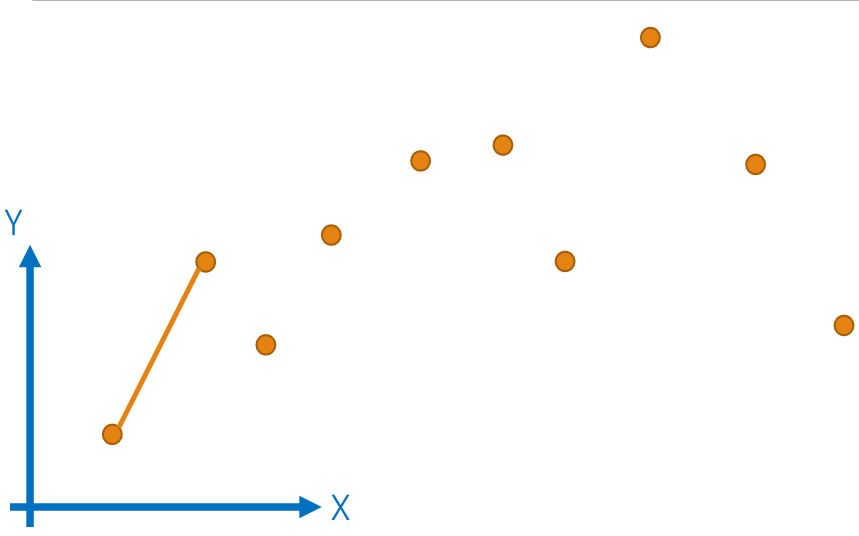
\includegraphics[width=0.24\textwidth]{afbeeldingen/first-convex}} 
		\subfigure[]{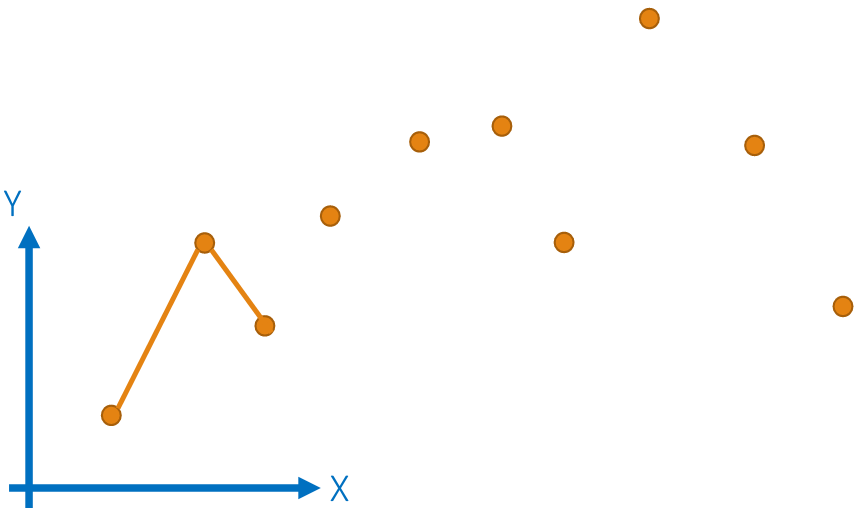
\includegraphics[width=0.24\textwidth]{afbeeldingen/second-convex}} 
		\subfigure[]{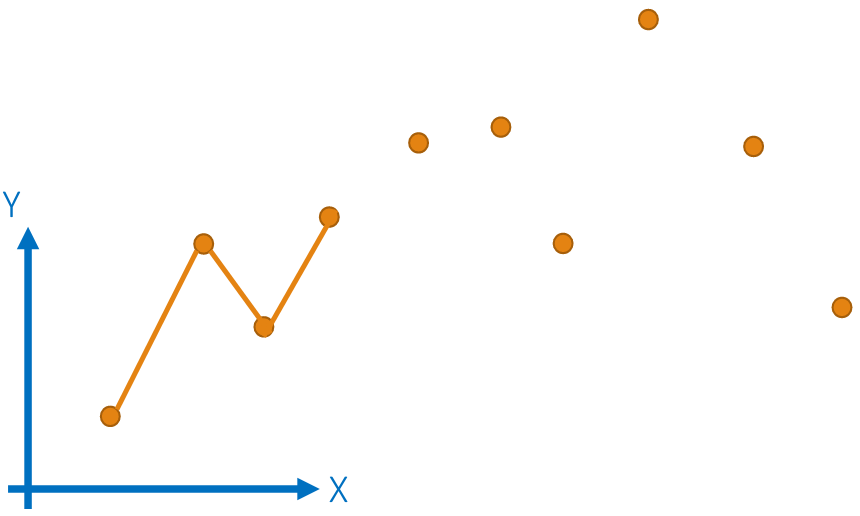
\includegraphics[width=0.24\textwidth]{afbeeldingen/third-convex}}
		\subfigure[]{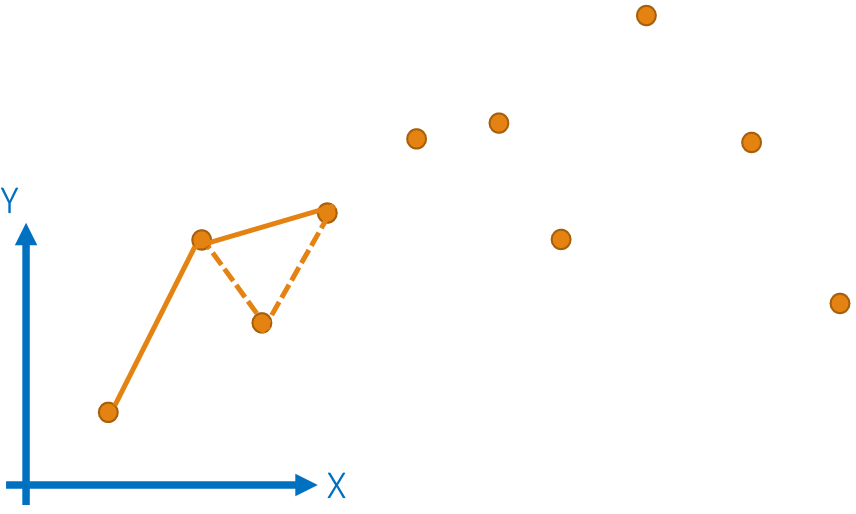
\includegraphics[width=0.24\textwidth]{afbeeldingen/fourth-convex}}
		\label{fig:incremental-example}
	\end{figure}
	Bij afbeelding c maken die punten duidelijk een linkerdraai, wat niet zou mogen voor een convex hull, dus zullen de twee edges verwijderd worden en vervangen worden door de nieuwe. Dit zal voor heel het puntenwolk verdergaan voor de bovenste helft. Voor duidelijkheid is hieronder nog de psuedocode
	\begin{figure}[h]
		\centering
		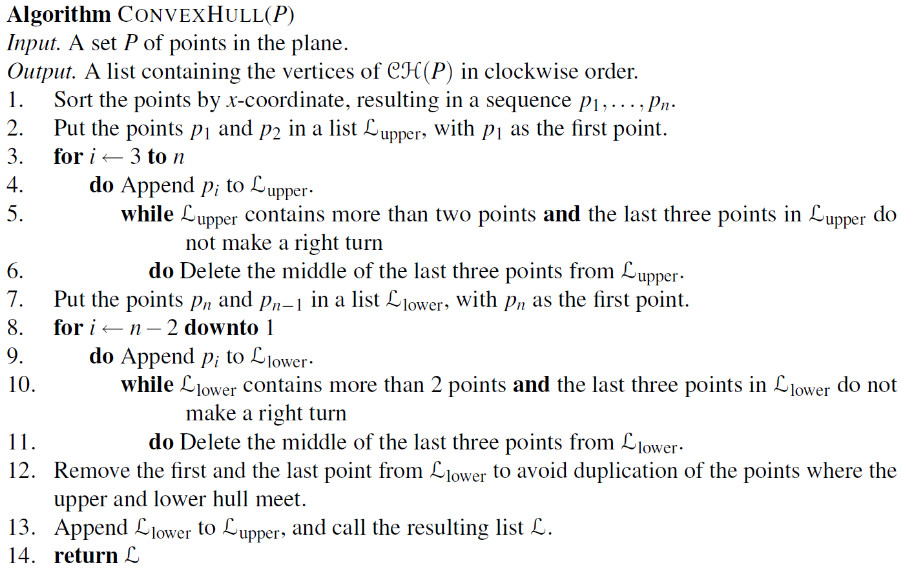
\includegraphics[width=0.9\linewidth]{afbeeldingen/convex-hull}
		\label{fig:convex-hull}
	\end{figure}

	De correctheid van het algoritme wordt bewezen d.m.v inductie: 
	\begin{itemize}
		\item Juiste bovengrens wordt berekend ${p_1, p_2}$
		\item Veronderstel dat we de juiste bovengrens berekend hebben voor ${p_1, p_2, ..., p_{i-1}}$
		\begin{itemize}
			\item $p_i$ toevoegen aan bovengrens - nieuwe bovengrens ligt boven de oude bovengrens
			\item Liggen alle punten ${p_1, p_2, ..., p_i}$ die niet behoren tot de bovengrens, beneden die bovengrens?
			\item Omwille van inductie tot $p_{i-1}$, kan enige mogelijkheid zijn dat een punt tussen $p_{i-1}$ en $p_i$ boven de bovengrens ligt, maar dit is onmogelijk, vermits we punten in gesorteerde volgorde behandelen. 
		\end{itemize}
	\end{itemize}
	Voor de tijdscomplexiteit weten we dat het sorteren van de punten $O(n\log(n))$ zal zijn terwijl voor de rest van het algoritme, we hoogstens één keer over elk punt zullen lopen, wat een tijdscomplexiteit geeft van $O(n)$. De totale tijdscomplexiteit van dit algoritme is dus \(O(n) + O(n\log(n)) = O(n\log(n))\).
	
	Ook voor dit algoritme zijn er speciale gevallen: wat als punten collineair zijn, wat met punten die hetzelfde x-coordinaat hebben en wat als er afrondingsfouten zijn in de hoeken. Dit kan allemaal opgelost worden met extra statements, maar dat geeft een lelijker algoritme. 
	
	
	\subsection{Graham's scan}
	Graham's scan zal niets aan het maken van de convex hull veranderen, maar zal het sorteren aanpassen. De punten zullen gesorteerd worden volgens poolhoek rond laagste meest linkse punt. Na het sorteren zullen de punten volgens de hoek overlopen worden om dan het verdere incrementeel algoritme toe te passen. De eerste van twee afbeeldingen bij Jarvis' march is een goede representatie van hoe de punten gesorteerd worden. 
	
	De tijdscomplexiteit is als volgt te bepalen. Het bepalen van het laagste punt is $O(n)$, het sorteren van de punten volgens punten zal $O(n\log(n))$ vragen en het overlopen zal zoals het vorige algoritme $O(n)$ vragen. De totale tijdscomplexiteit is dus $O(n\log(n))$. 
	
	
	\subsection{Jarvis's March}
	Jarvis' march zal beginnen zoals Graham's scan, beginnen met het uiterst links onderste punt en dan op poolhoeken sorteren, en zal die voor elk punt opnieuw doen. Dit wordt verduidelijkt door de onderstaande afbeeldingen; 
	
	\begin{figure}[h]
		\centering
		\subfigure[]{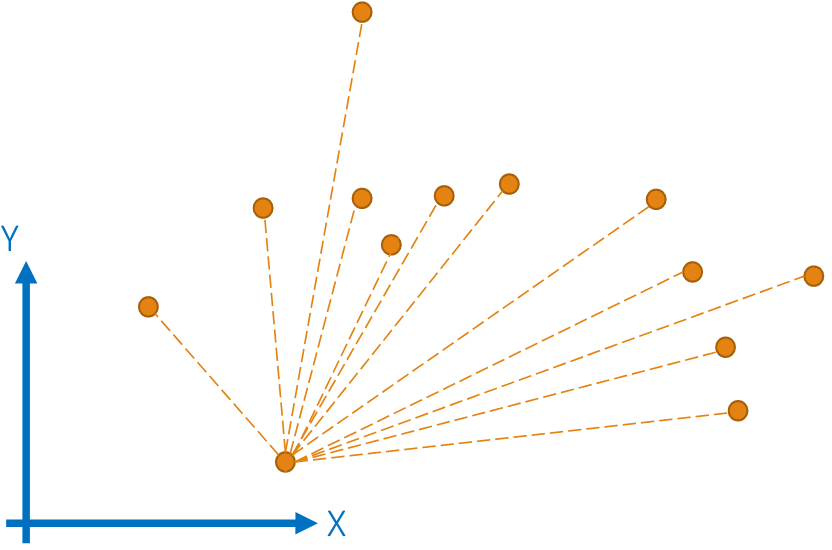
\includegraphics[width=0.45\textwidth]{afbeeldingen/first-jarvis}} 
		\subfigure[]{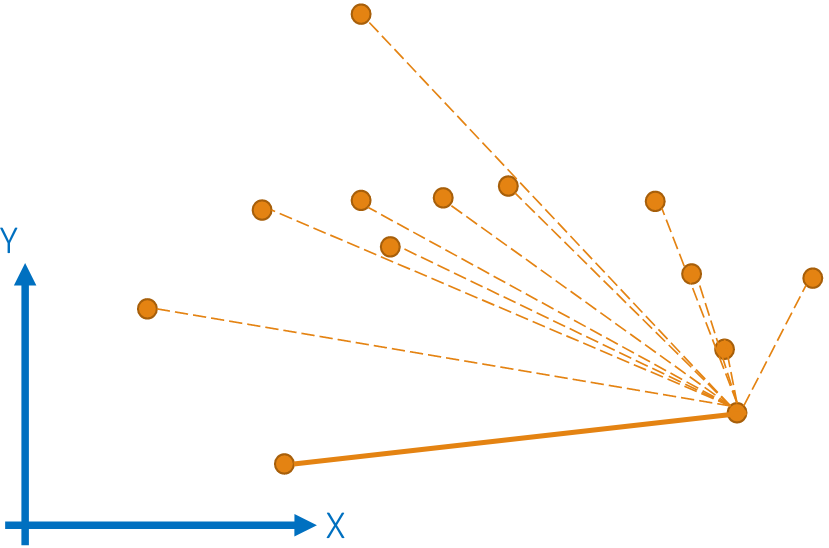
\includegraphics[width=0.45\textwidth]{afbeeldingen/second-jarvis}} 
		\label{fig:jarvis' example}
	\end{figure}

	Voor elk hoekpunt zal gekeken worden naar alle andere punten in de ruimte, hier voelen we aan dat in onze complexiteitsanalyse, we rekening zullen moeten houden met het aantal hoekpunten. Dit is het eerste algoritme waarbij we rekening houden met de output, wat resulteert in een \textit{output-afhankelijke tijdscomplexiteit}. Het aantal hoekpunten en dus het aantal elementen in de output zal in de tijdscomplexiteit $h$ zijn. Gezien we voor elk hoekpunt ongeveer alle andere punten moet overlopen, is de tijdscomplexiteit $O(n\cdot h)$.
	
	Dit algoritme zal dus bijna lineaire tijd hebben bij heel weinig hoekpunten, wat veel beter is dan graham's scan. Anderzijds kan het bijna een kwadratische tijdscomplexiteit worden als het aantal hoekpunten even groot wordt als het algemeen aantal punten. 
	
	Jarvis' march zal bij een klein aantal hoekpunten het logisch algoritme zijn terwijl graham's scan beter is voor een groter aantal. 
	
	%TODO navragen!
	

	\subsection{Verdeel-en-heers}
	Dit is een strategie die we al hebben zien terugkeren bij sorteeralgoritmes. We splitsen het probleem op, we lossen de kleinere problemen op en dan combineren we de oplossingen. De recursie stopt als de verzameling triviaal klein wordt. De tijdscomplexiteit van zo'n algoritmes is vaak $O(n\log(n))$. 
	
	Een manier is om de puntenwolk telkens willekeurig te verdelen en dan de twee convex omhullenden telkens te mergen op de meest extreme punten. Dit lijkt al heel goed, maar willekeurig kan ook heel slechte algoritmes brengen, dus is dit niet altijd het meest ideale. 
	
	Een tweede manier is om de puntenwolk telkens perfect in twee te verdelen volgens de x-coördinaten. De merge-operatie is dan telkens een bovenraaklijn en een onderraaklijn zoeken om deze te verbinden en nog steeds een convex omuhllende te verkrijgen. Deze onder- en bovenbrug is niet altijd het onderste en/of bovenste punt van een puntenwolk, hier bestaat dus een algoritme voor: 
	
	\begin{figure}[h]
		\centering
		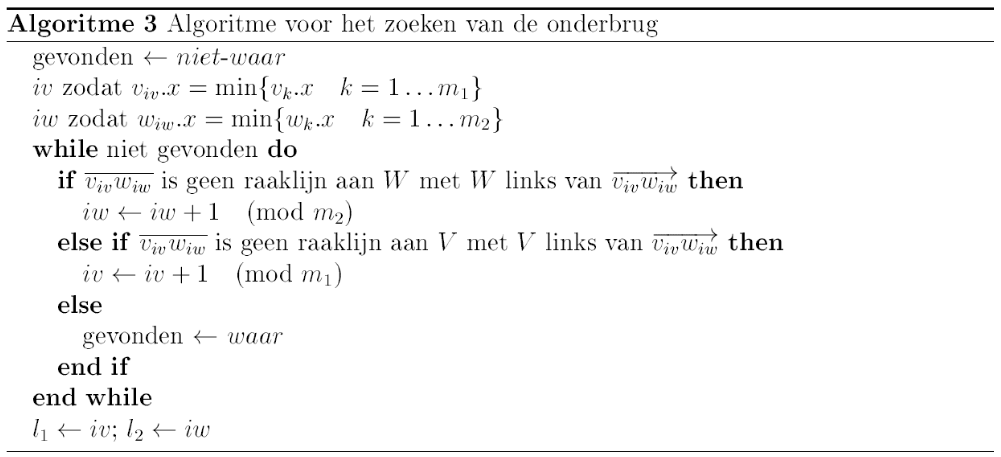
\includegraphics[width=0.9\linewidth]{afbeeldingen/verdeel-en-heers-convex}
		\label{fig:verdeel-en-heers-convex}
	\end{figure}
	%TODO verdere uitleg zoeken want hier zou mondelinge uitleg best ook bijkomen
	
	
	\section{Les 2: Intersecties van lijnstukken}
	\subsection{Brute Force algoritme}
	\subsection{Doorlooplijn algoritme}
	\subsection{Doubly-connected edge 	list}
	\section{Les 3: }
	\section{Les 4: }
	\section{Les 5: }
	\section{Les 6: }
	\section{Les 7: }
	\section{Les 8: }
	\section{Les 9: }
	\section{Les 10: }
	\section{Les 11: }
\end{document}